\section{Эксперименты}

Был проведён ряд экспериментов, которые позволили оценить некоторые параметры инструмента.

Во всех приведённых ниже тестах грамматики описываются на языке YARD. Так же предположим, что у нас есть сторонний лексический анализатор со следующим набором лексем:
\begin{itemize}
  \item PLUS = '+'
  \item MINUS = '-'
  \item DIV = '/'
  \item MULT = '*'
  \item LEFT = '('
  \item RIGHT = ')'
  \item NUMBER = (0..9)+
  \item SEMICOLON = ';'
\end{itemize}

По этому будем предполагать, что на вход инструменту поступает поток лексем.


\subsection{Работа с однозначными грамматиками} 

Необходимо показать, что по однозначной грамматике строится инструмент имеющий линейную временную сложность. Для этого необходимо оценить количество действий LR-автомата, совершаемых при распознавании цепочки. Оно должно линейно зависеть от длинны входа.

В нашем случае операции LR-автомата -- это вызовы функций $parse$ и $climb$. То есть нам надо оценить зависимость количества вызовов этих функций от длинны входной цепочки.


Возьмём грамматику:

\begin{verbatim}
f : <n:string>=NUMBER {float n}
  | l=LEFT <expr:float>=e r=RIGHT {expr};  
  
t : <l:float>=t op=(MULT {( * )} | DIV {( / )} ) <r:float>=f {op l r}
  | res=f {res};
  
e : res=t {res}
  | <l:float>=e op=(PLUS {( + )} | MINUS {( - )} ) <r:float>=t {op l r}; 
  
+s: res=e {res};
\end{verbatim}

Возьмём n = "`2*3"' и проведём тесты для строк n'+'kn, kn = $concat \ '\!+' [\underbrace {n,n, ... , n}_\text{k раз}] | k = 0..99 $. В результате получим график~\ref{fig:assimpt}, где по оси Ox откладывается k, а по Oy -- количество вызовов. Видно, что зависимость количества действий LR-автомата линейно зависит от длины входной цепочки.

\begin{center}
  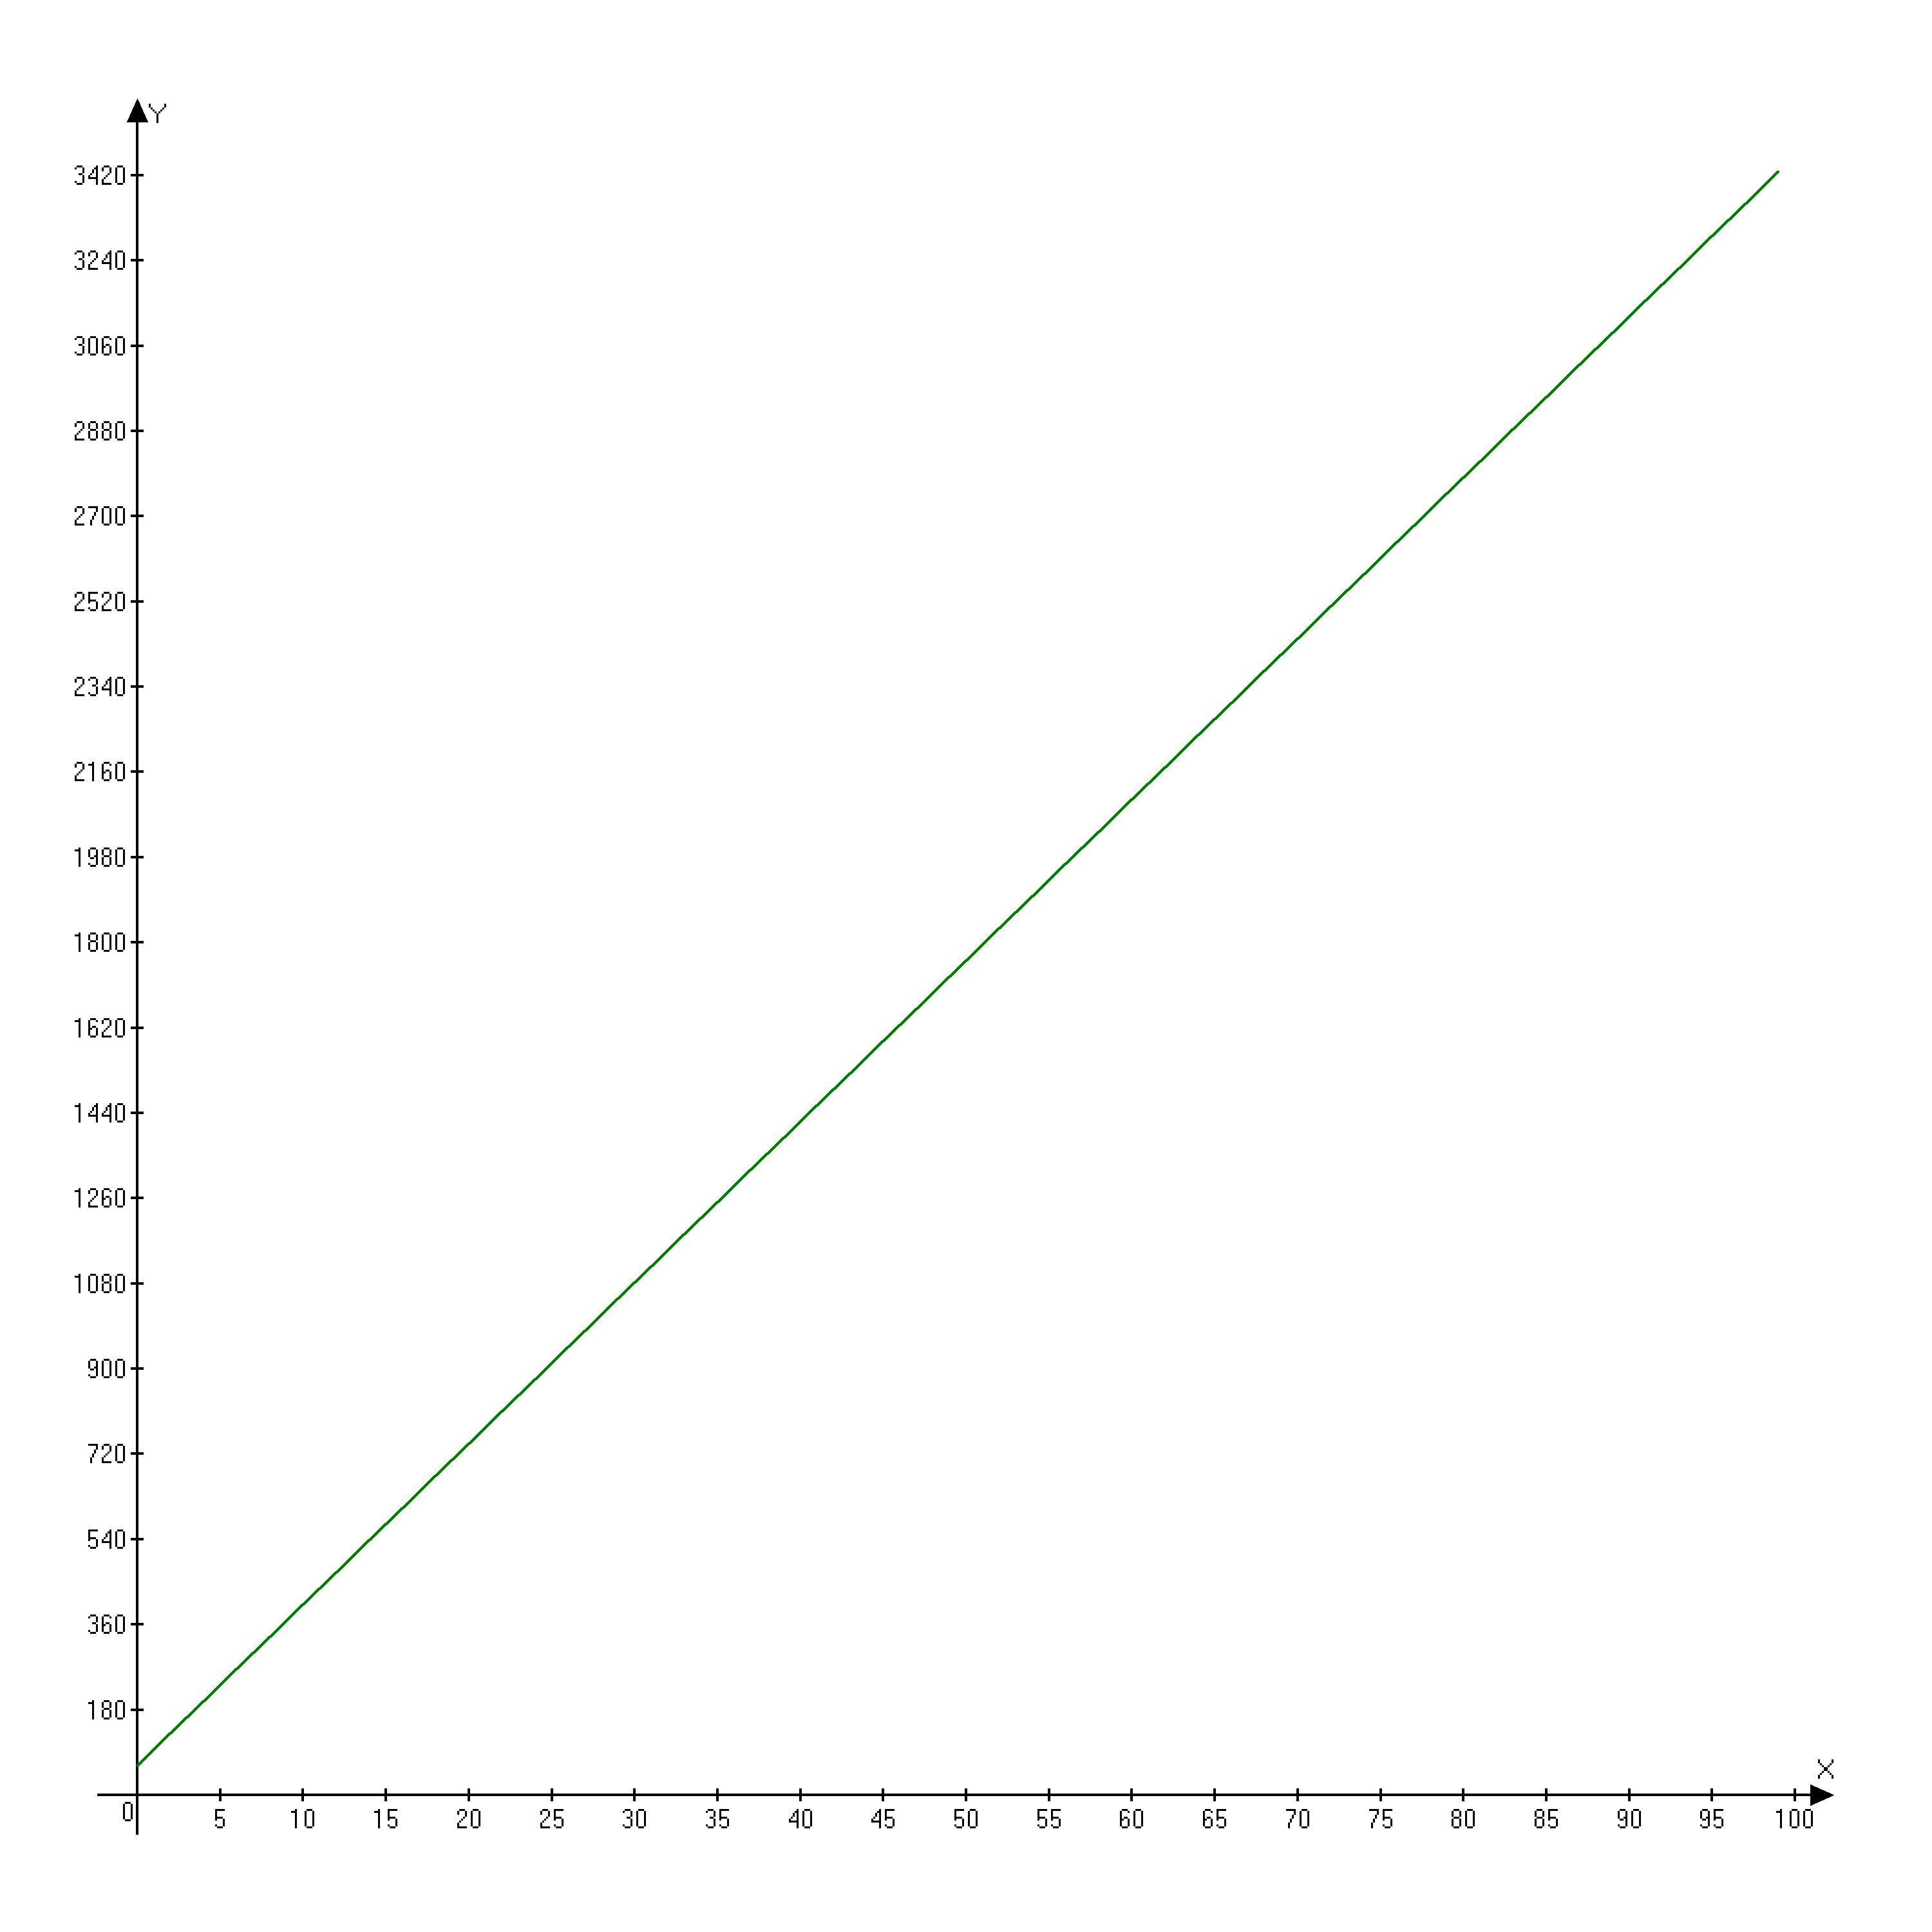
\includegraphics[height = 15cm]{Pictures/CallCount_18.jpg} 
	\captionof{figure}{Зависимость количества действий LR-автомата от длинны входной цепочки.}
	\label{fig:assimpt}
\end{center}


\subsection{ Возможность работы с неоднозначными грамматиками} 

Для этого необходимо проверить, что при неоднозначной грамматике инструмент возвращает все возможные варианты вывода входной строки. В качестве примера была взята следующая грамматика:

\begin{verbatim}
+s : e;
e : e (PLUS | MINUS | MULT | DIV  ) e 
  | LEFT e RIGHT 
  | NUMBER ;
\end{verbatim}

Эта грамматика описывает арифметические выражения без приоритетов. Очевидно, что данная грамматика содержит неоднозначности. 

Рассмотрим несколько примеров входных цепочек:
\begin{itemize}

  \item Пусть тестовая строка: "`1+2"'. Соответсвенно, список лексем: \verb|[NUMBER; PLUS; NUMBER]|. Существует единственное дерево вывода для данной цепочки:

    \begin{centering}

      \begin{dot2tex}[dot]
       digraph g
       {
          S [label = "S"]
          e1 [label = "e"]
          e2 [label = "e"]
          plus [label = "PLUS"]
          e3 [label = "e"]
          num1 [label = "NUMBER"]
          num2 [label = "NUMBER"]
          S -> e1
          e1 -> e2
          e1 -> plus
          e1 -> e3
          e2 -> num1
          e3 -> num2
       }
      \end{dot2tex}

    \end{centering}

Инструмент так же возвращает единственное дерево:
\begin{verbatim}
<NODE name="S">
        <NODE name="e">
            <NODE name="e">
                <LEAF name="NUMBER"/>
            </NODE>
            <LEAF name="PLUS"/>
            <NODE name="e">
                <LEAF name="NUMBER"/>
            </NODE>
        </NODE>
</NODE>
\end{verbatim}

\item Строка: "`1+2+3"'. Список лексем: \verb|[NUMBER; PLUS; NUMBER; PLUS; NUMBER]|. Для данной цепочки существует два дерева вывода и инструмент возвращает оба:
\begin{verbatim}
<NODE name="s">
    <NODE name="e">
        <NODE name="e">
            <NODE name="e">
                <LEAF name="NUMBER"/>
            </NODE>
            <LEAF name="PLUS"/>
            <NODE name="e">
                <LEAF name="NUMBER"/>
            </NODE>
        </NODE>
        <LEAF name="PLUS"/>
        <NODE name="e">
            <LEAF name="NUMBER"/>
        </NODE>
    </NODE>
</NODE>

<NODE name="s">
    <NODE name="e">
        <NODE name="e">
            <LEAF name="NUMBER"/>
        </NODE>
        <LEAF name="PLUS"/>
        <NODE name="e">
            <NODE name="e">
                <LEAF name="NUMBER"/>
            </NODE>
            <LEAF name="PLUS"/>
            <NODE name="e">
                <LEAF name="NUMBER"/>
            </NODE>
        </NODE>
    </NODE>
</NODE>
\end{verbatim}
	
\end{itemize}
	
Таким образом, инструмент строит все возможные варианты вывода в случае, если грамматика неоднозначна.

\subsection{Возможность работы с EBNF-грамматиками} 

Основные конструкции регулярных выражений, для которых необходимо провести проверку: последовательность, альтернатива, замыкание. Важно обратить внимание на соответствие получаемого дерева вывода ожидаемому результату. Для этого нужно проверить соответствие дерева вывода входной грамматике. В нём не должно быть новых терминалов и нетерминалов.

Для примера возьмём следующую грамматику:
\begin{verbatim}
f : NUMBER 
  | LEFT e RIGHT ;  
  
t : t (MULT | DIV ) f 
  | f ;
  
e : t 
  | e (PLUS | MINUS )t; 
  
+s: e (SEMICOLON e )* ;

\end{verbatim}

Данная грамматика описывает список арифметических выражений, разделённых точкой с запятой. Видно, что в ней используются все заявленные конструкции регулярных выражений (последовательность, альтернатива, замыкание).

Пусть на вход подаётся строка: "`2*3; 3*4; 5*5"'. Инструмент построит следующее дерево вывода:
\begin{verbatim}
<NODE name="s">
    <NODE name="e">
        <NODE name="t">
            <NODE name="t">
                <NODE name="f">
                    <LEAF name="NUMBER"/>
                </NODE>
            </NODE>
            <LEAF name="MULT"/>
            <NODE name="f">
                <LEAF name="NUMBER"/>
            </NODE>
        </NODE>
    </NODE>
    <LEAF name="SEMICOLON"/>
    <NODE name="e">
        <NODE name="t">
            <NODE name="t">
                <NODE name="f">
                    <LEAF name="NUMBER"/>
                </NODE>
            </NODE>
            <LEAF name="MULT"/>
            <NODE name="f">
                <LEAF name="NUMBER"/>
            </NODE>
        </NODE>
    </NODE>
    <LEAF name="SEMICOLON"/>
    <NODE name="e">
        <NODE name="t">
            <NODE name="t">
                <NODE name="f">
                    <LEAF name="NUMBER"/>
                </NODE>
            </NODE>
            <LEAF name="MULT"/>
            <NODE name="f">
                <LEAF name="NUMBER"/>
            </NODE>
        </NODE>
    </NODE>
</NODE>
\end{verbatim}

Видно, что в дереве нет дополнительных нетерминалов или терминалов. Присутствуют только те, которые описаны в пользовательской грамматике, то есть инструмент реализует непосредственную поддержку EBNF-грамматик.


\subsection{Поддержка s-атрибутных грамматик}

 Необходимо показать корректность вычисления атрибутов в случае неоднозначной грамматики. Для этого необходимо, чтобы операции с побочными эффектами работали корректно (например, проверить, что при наличии в атрибутах действия печати на экран, на экран  не выводится лишней информации). Так же необходимо показать возможность вычисления атрибутов в случае расширенной контекстно-свободной  грамматики. 

Рассмотрим следующую грамматику:
\begin{verbatim}
+ s : t {printfn "\n reduce t rule \n"};
t : a {printfn "\n reduce a rule \n"};
t : b {printfn "\n reduce b rule \n"};
a : PLUS NUMBER {printfn "\n visit a rule \n"};
b : PLUS NUMBER SEMICOLON {printfn "\n visit b rule \n"};
\end{verbatim}

Пусть дана строка: "`+1;"' Для неё возможно две "`попытки"' \ вывода в данной грамматике (попытка свернуть правило \verb|a| и попытка свернуть правило \verb|b|), но только одна из них завершится удачно. В качестве атрибутов указано действие с побочным эффектом -- печать на экран. Важно убедиться, что на экран будет выведено только то, что соответствует удачному варианту разбора.

В процессе работы инструмента можно увидеть, что попытка свернуть по правилу \verb|a|  действительно была. Это видно, например, в трассе:
\begin{verbatim}
...
  trees:
         <NODE name="t">
            <NODE name="a">
                <LEAF name="PLUS"/>
                <LEAF name="NUMBER"/>
            </NODE>
        </NODE>
...
\end{verbatim}

Однако на экране будет напечатано следующее:
\begin{verbatim}
 visit b rule

 reduce b rule

 reduce t rule
\end{verbatim}

Печати, связанной с правилом  \verb|a| нет. Можно так же проверить дерево вывода. Инструмент получил единственное дерево:
\begin{verbatim}
<NODE name="s">
    <NODE name="t">
        <NODE name="b">
            <LEAF name="PLUS"/>
            <LEAF name="NUMBER"/>
            <LEAF name="SEMICOLON"/>
        </NODE>
    </NODE>
</NODE>
\end{verbatim}

Таким образом, в случае, если грамматика неоднозначна, работа с действиями с побочными эффектами происходит корректно. 

Теперь проверим работу вычисления атрибутов для EBNF-грамматик. Для этого рассмотрим следующую грамматику:

\begin{verbatim}
f : <n:string>=NUMBER {float n}
  | l=LEFT <expr:float>=e r=RIGHT {expr};  
  
t : <l:float>=t op=(MULT {( * )} | DIV {( / )} ) <r:float>=f {op l r}
  | res=f {res};
  
e : res=t {res}
  | <l:float>=e op=(PLUS {( + )} | MINUS {( - )} ) <r:float>=t {op l r}; 
  
+s: r = e lst = (SEMICOLON  l = e {l})* 
    {List.iter (printfn "result = %A \n") (r::lst)};
\end{verbatim}

На вход подаём строку: "`2*3; 3*4; 5*5"' . На выходе получаем следующий результат:

\begin{verbatim}
result = 6.0

result = 12.0

result = 25.0
\end{verbatim}

То есть инструмент поддерживает работу с s-атрибутами при непосредственной поддержке EBNF-грамматик.

Так же, в ходе этого эксперимента было выявлено, что предложенное решение, в котором явным образом строится дерево вывода и для каждого правила строится своя семантическая функция, оказывается удобным. С одной стороны, это позволяет упростить отладку, потому, что всегда можно проверить правильность построения дерева и в отладчике просто проконтролировать вычисление в конкретном узле (мы знаем при свёртке какого правила появился этот узел и знаем какая функция должна вычисляться). С другой -- прямой доступ к лесу вывода позволяет совершать с ним дополнительные операции.  Дополнительную фильтрацию или, например, печать, что оказалось полезным при получении результатов экспериментов (печать XML-представления деревьев). 
